\documentclass[modern,letterpaper]{aastex61}

% to-do list
% ----------
% - add items here
% style notes
% -----------
% - This file generates by Makefile; don't be typing ``pdflatex'' or some bullshit.
% - Line break between sentences to make the git diffs readable.
% - Use \, as a multiply operator.
% - Reserve () for function arguments; use [] or {} for outer shit.
% - Use \sectionname not Section, \figname not Figure, \documentname not Article or Paper or paper.

% packages
\definecolor{cbblue}{HTML}{3182bd}
\usepackage{microtype}  % ALWAYS!
\usepackage{amsmath,amssymb}
\usepackage{tikz}
\usepackage{aas_macros}
\hypersetup{backref,breaklinks,colorlinks,urlcolor=cbblue,linkcolor=cbblue,citecolor=black}
\graphicspath{{.}{figures/}{../notebooks/plots/}}

% define macros for text
\newcommand{\project}[1]{\textsl{#1}}
\newcommand{\acronym}[1]{{\small{#1}}}
\newcommand{\hipparcos}{Hipparcos}
\newcommand{\gaia}{\project{Gaia}}
\newcommand{\rave}{\project{\acronym{RAVE}}}
\newcommand{\apogee}{\project{\acronym{APOGEE}}}
\newcommand{\tmass}{\project{\acronym{2MASS}}}
\newcommand{\documentname}{Article}
\newcommand{\sectionname}{Section}
\newcommand{\figname}{Figure}
\newcommand{\eqname}{Equation}
\newcommand{\dr}{\acronym{DR1}}
\newcommand{\tgas}{\acronym{TGAS}}
\newcommand{\etal}{\textit{et al}.}

\newcommand{\objname}{moving group}
\newcommand{\groupTen}{Group 10}
\newcommand{\groupSixteen}{Group 16}

% define macros for math
\newcommand{\given}{\,|\,}
\newcommand{\normal}{{\mathcal{N}}}
\newcommand{\uniform}{{\mathcal{U}}}
\newcommand{\dd}{\mathrm{d}}
\newcommand{\transp}[1]{{#1}^{\!\mathsf{T}}}
\newcommand{\inv}[1]{{#1}^{-1}}
\newcommand{\bs}[1]{\boldsymbol{#1}}
\newcommand{\vperp}{\bs{v}^\perp}
\newcommand{\propm}{\bs{\mu}}
\newcommand{\mat}[1]{\mathbf{#1}}
\renewcommand{\vec}[1]{\bs{#1}}
\newcommand{\kms}{\ensuremath{\rm km~s^{-1}}}
\newcommand{\msun}{{\rm M}_\odot}
\newcommand{\data}{\mathrm{data}}
\newcommand{\snr}{[S/N]_\varpi}
\newcommand{\eye}{\mathbb{I}}
\newcommand{\absdvtan}{\ensuremath{|\Delta\vec v_\mathrm{t}|}}
\newcommand{\estimates}{\ensuremath{\{\hat{\varpi_i},\hat{\mu_{\alpha,i}},\hat{\mu_{\delta,i}},\hat{v_{r,i}}\}}}

\definecolor{crimson}{rgb}{0.79, 0.0, 0.09}
\newcommand{\todo}[1]{{\color{crimson}#1}}

\newcommand{\groupDistanceEstimate}{\ensuremath{100~\mathrm{pc}}}
\newcommand{\groupAgeEstimate}{\ensuremath{500~\mathrm{Myr}}}
\newcommand{\totalNumberOfCandidates}{\ensuremath{29}}
\newcommand{\meanVelocityOpt}{\ensuremath{(u_x,\,u_y,\,u_z) = (-3.9,\,7.0,\,-3.8)~\kms}}
\newcommand{\sigVelocityOpt}{\ensuremath{0.42~\kms}}

\begin{document}\sloppy\sloppypar\raggedbottom\frenchspacing % trust me

\title{
  Rediscovery of a nearby young moving group
}

\author[0000-0001-7790-5308]{Semyeong Oh \etal}
\affiliation{Department of Astrophysical Sciences,
             Princeton University, Princeton, NJ 08544, USA}

\correspondingauthor{Semyeong Oh}
\email{semyeong@astro.princeton.edu}

\begin{abstract}

  We characterize a nearby (\todo{$d \approx \groupDistanceEstimate$}),
  young (\todo{age $\approx \groupAgeEstimate$}) moving group using \gaia\ DR 1
  astrometry and photometric and spectroscopic data from the literature.
  This group, which notably includes \todo{81 Uma},
  partially overlaps with the putative new open cluster composed of
  seven A-type stars by \citet{1977ATsir.969....7L} but its status
  was dubious due to ...
  Here, we show that three of these stars are part of a larger comoving group
  that have \totalNumberOfCandidates\ candidate members.
  We model the proper motions of the candidate members with a simple
  isotropic Gaussian velocity distribution, and find that
  the velocity dispersion is very small (\todo{X}) verifying
  that they are comoving.
  Because the group spans a large area on sky, the astrometric radial velocities
  of individual stars based on the model is determined with \todo{this precision}.
  We discuss ....

\end{abstract}

\section{Introduction} % (fold)
\label{sec:introduction}

Stars form in group, and remain coherent in their kinematics for a period of
time that, most importantly, depends on the mass of the initial mass of the
molecular clouds. Thus, looking for comoving groups of stars is an efficient
way to find moving groups of presumably single stellar population.

Simple stellar populations are useful for many things. Based on the assumption
that a group of stars have the same age, many of the stellar parameters can be
more precisely inferred. Particularly, stellar ages, which are important yet
challenging to constrain for a single star, can be pinned down to
\todo{$approx 10$\%} precision.

Young, hot stars are primary targets for discovering planets and brown dwarfs
with direct imaging.

Here, we report extended analysis and spectroscopic characterization of two
nearby moving groups.


\begin{figure}[ht]
  \centering
  \includegraphics[width=0.95\linewidth]{figures/g10_3panels.pdf}
  \caption{\label{fig:g10_3panels}
    Distribution of 29 stars in \groupTen\ on sky (a),
    proper-motion space (b), and color-magnitude space (c).
    In panel (a), the lines connecting pairs of stars show the comoving pairs
    that constitute this group (connected component) from
    \citet{2017AJ....153..257O}.
    In panel (b), the ellipses show the $2\sigma$ covariances of the \tgas\
    data.
    In panel (c), MIST isochrones of solar-metallicity for ages of 100~Myr,
    500~Myr, and 1~Gyr are plotted.
  }
\end{figure}


\subsection{Previous identifications}
\label{subsec:history}

Moving group identifications are often scattered throughout the literature. We
reviewed a (non-exhaustive) bibliography associated with all \tgas\ sources in
\groupTen\ from our previous selection \citep{2017AJ....153..257O} using the
Simbad database, and note previous identifications of this group.

Some A-type stars that were selected in \citet{2017AJ....153..257O} as potential
members of \groupTen,
HIP 66198 (81 Uma), HIP 67231 (84 Uma), and HIP 67005, are part of an open cluster
suggested by \citet{1977ATsir.969....7L} and dubbed Latyshev 2 by Archinal \& Hynes.
The reality of the putative cluster, composed of 7 A-type stars
HIP 66198,
HIP 67231,
HIP 67005,
HIP 67848,
HIP 66738,
TYC 3851-606-1,
TYC 3469-497-1,
was dismissed in a recent review by \citet{2016IAUS..314...21M}.
However, here we report that there indeed is a comoving group containing
some of the stars in Latyshev 2, and that we have identified the lower-MS stars
in \tgas, demonstrating its physical reality more convincingly.
We found that two of the \hipparcos\ stars in Latyshev 2,
HIP 67848 (86 Uma) and HIP 66738 (83 Uma),
were missing in the \tgas\ catalog which was the parent sample of our previous search while
their proper motions have been determined by \hipparcos.
Motivated by this, we looked for any bright members of both groups that we
may have missed using \hipparcos\ stars that are not present in \tgas\ (\todo{see section X}).

% section introduction (end)

\section{Observation}
\label{sec:observation}

\subsection{Target Selection}
\label{sub:target_selection}

We re-examined the network of co-moving pairs studied in \citealt{2017AJ....153..257O} by
lowering the threshold of the marginalized likelihood ratios to be more inclusive.
For $\ln{\mathcal{L}_1}/{\mathcal{L}_2}>2$, we find that this group,
identified as group id 10 in \citealt{2017AJ....153..257O}, is extended to 45 potential members.

table for targets and observation




% \section{Searching lower main sequence in GPS1}
% \label{sec:searching_lower_main_sequence_in_gps1}

% \begin{figure}[htpb]
%   \centering
%   \includegraphics[width=0.8\linewidth]{g0_pm.pdf}
%   \caption{
%     Group 0 (the Pleiades; black circles) stars in proper-motion space. The
%     stars are well-separated from the distribution of the background stars
%     within the same patch of the sky. The Blue box indicates the proper motion
%     cuts applied to select stars from GPS1 catalog.
%   }
%   \label{fig:g0_pm}
% \end{figure}

% \begin{figure}[htpb]
%   \centering
%   \includegraphics[width=0.95\linewidth]{g0_gps1.pdf}
%   \caption{
%     Potential members of the Pleiades selected from GPS1. These are 2095 stars
%     that are within 15 degrees from the center (median RA, Dec) and have proper
%     motions within the cuts indicated in Figure 1 . The line in each panel is
%     the isochrone from MIST model. In the top left panel, the purple shade for
%     the (pre-)main sequence shows the span from using the minimum and the
%     maximum parallax values. In order to shift the model magnitudes to observed
%     magnitudes, a point-estimate distance of 1/(median parallax) is used.
%   }
%   \label{fig:g0_gps1}
% \end{figure}

% We first find the lower main-sequence stars of the Pleiades (Group 0) using the
% GPS1 data. The Pleiades is chosen as it is clearly very separated in
% proper-motion space alone (Figure 1). We apply a simple cut in proper motions
% to be within the minimum and maximum values of the TGAS-selected Group 0
% members (indicated with a blue box in Figure 1, and query 15 degrees around the
% center (median RA, Dec) of the group. There are 2095 stars satisfying the cuts
% in the GPS1 catalog. Figure 2 shows their distribution in color-magnitude
% diagrams using Gaia, 2MASS, and PanSTARRS photometry with MIST (\citealt{2016ApJ...823..102C}).

% We first find the lower main-sequence stars of the Pleiades (Group 0) using the
% GPS1 data. The Pleiades is chosen as it is clearly very separated in
% proper-motion space alone (Figure~\ref{fig:g0_pm}). We apply a simple cut in
% proper motions to be within the minimum and maximum values of the TGAS-selected
% Group 0 members (indicated with a blue box in Figure~\ref{fig:g0_pm}, and query 15
% degrees around the center (median RA, Dec) of the group. There are 2095 stars
% satisfying the cuts in the GPS1 catalog. Figure~\ref{fig:gps_gps1} shows their
% distribution in color-magnitude diagrams using Gaia, 2MASS, and PanSTARRS
% photometry with the MIST isochrone of solar metallicity and 8.5~Myrs. Although
% there is clearly contamination from background stars with this simple cuts, the
% expected over-density in the low main-sequence is well recovered (and possibly
% a few suspect WDs on the cooling sequence!).

% However, there is a noticeable disagreement between the MIST isochrone and the
% data in the red colors in that the model isochrone predict bluer colors than
% observed. This is a known problem due to incomplete spectral library for
% generating stellar spectral energy distributions from physical parameters
% (Choi+2016).


% We searched the Simbad (\citealt{2000A&AS..143....9W}) database for existing
% radial velocity measurements of the candidate members

\section{Modelling as a group}

Although the original selection was done by selecting comoving pairs, we can
also model the proper motions of stars in a group (connected component) as drawn
from a single mean velocity with a small dispersion.
\todo{rephrase:
This is essentially the moving cluster method or convergent point method,
but instead of taking procedural steps to confirm or find the existence of a
convergent point, we wish to take forward modelling approach with a probabilistic basis.}
\todo{CITE: Lindegren etc.}

The components of the model are:
\begin{itemize}
  \item We assume that the velocity $\vec{v}_i$ of the star $i$ is drawn from
    a single Gaussian component with mean (group) velocity $\vec{u}$ and
    an isotropic dispersion $\sigma_{u}$:
    $$\vec{v}_i \sim \normal(\vec{u},\,\sigma_{u}).$$
    Then, the proper motion of star $i$ is $\mat{M}_i(\alpha_i,\,\delta_i)\vec{v}_i$ where
    $\mat{M}_i$ is the rotation matrix that transforms the equatorial rectangular coordinates
    \footnote{The choice of this coordinate system is arbitrary. Many of the studies on
      moving grouops in the Solar neighborhood choose the Galactic coordinates which additionally
      depends on $(\alpha_\mathrm{GC},\,\delta_\mathrm{GC})$.
    }
    to the tangential coordinates at the location $(\mathrm{R.A.},\,\mathrm{Decl.}) = (\alpha_i,\,\delta_i)$.

  \item We assume that the noise model for the \gaia\ data is Gaussian, and
    the covariance matrix $C_i$ is given and fixed:
    $$(\tilde\varpi_i,\,\tilde\mu_{\alpha,i}^*,\,\tilde\mu_{\delta,i}) \sim
      \normal((\varpi_i,\,\mu_{\alpha,i}^*,\,\mu_{\delta,i}),\,C_i)$$

  \item \emph{Priors}: We assume a constant density prior ($p(r) \propto r^2$) and a Gaussian
    prior with 30~\kms\ dispersion for the mean velocity of the group.
    For the dispersion $\sigma_u$, we assume a uniform prior in $[0,\,50)$.
\end{itemize}


\begin{figure}
  \centering
  \includegraphics[width=0.9\linewidth]{quiver_pm.pdf}
  \caption{Proper-motion vectors (left) and residual proper motion vectors (right)
    for 29 stars in \groupTen\ on sky.
    The residuals are from subtracting the projected mean velocity (\todo{see section X}).
    The length scale in each panel marked in the upper left corner.
  }
  \label{fig:quiver_pm}
\end{figure}

\begin{figure}
  \centering
  \includegraphics[width=0.9\linewidth]{isotropic_single_mc.pdf}
  \caption{
    Posterior distribution of the mean velocity $\vec{u} = (u_x,\,u_y,\,u_z)$ and
    isotropic dispersion $\sigma_u$.
    Note priors.
  }
  \label{fig:fit}
\end{figure}

\begin{figure}
  \centering
  \includegraphics[width=0.9\linewidth]{rv_ra_id.pdf}
  \caption{
    Comparing astrometric radial velocities (blue patches) to
    measurements available from the literature (black circles).
    The stars are spread along their R.A. in the vertical direction.
    The blue patches for each star shows the posterior distribution
    of the star's radial velocity predicted from the proper motions of
    all stars in the group.
    All available measurements removing duplicated exact values from
    the literature are shown.
    In general, the the predicted astrometric RVs match one or more
    available measurements for a star.
  }
  \label{fig:rv_ra_id}
\end{figure}

We first do an optimization using L-BFGS algorithm starting from the
initial values $d_{i,0} = 1/{\tilde \varpi_0}$, a random mean velocity $\vec{u}_0$
drawn from the prior distribution, and $\sigma_u=10$~\kms.
We find that the optimized mean velocity is \meanVelocityOpt\ and the dispersion \sigVelocityOpt.
We then sample the posterior distribution of $d_i$, $\vec{u}$ and $\sigma_u$ starting
from this optimum.
\figname~\ref{fig:quiver_pm} and \figname~\ref{fig:fit} summarizes
the fit result.


Because this group spans a large area on sky,
the geometric constraint on the radial velocities of the stars is interesting.
\todo{Figure:radial velocities}
We compare this to a compilation of radial velcoity measurements from the literature.
We searched the Simbad database ...





\section{Discussion}
\label{sec:discussion}

% \begin{deluxetable}{cccccccc}
\tablecaption{Candidate members of the new moving group}
\tablehead{\colhead{Id} & \colhead{RA} & \colhead{Dec} & \colhead{$d$} & \colhead{$\mu_\alpha^*$} & \colhead{$\mu_\delta$} & \colhead{$G$} & \colhead{$G-J$}\\ \colhead{ } & \colhead{$\mathrm{{}^{\circ}}$} & \colhead{$\mathrm{{}^{\circ}}$} & \colhead{$\mathrm{pc}$} & \colhead{$\mathrm{mas\,yr^{-1}}$} & \colhead{$\mathrm{mas\,yr^{-1}}$} & \colhead{$\mathrm{mag}$} & \colhead{$\mathrm{mag}$}}
\startdata
TYC 4164-274-1 & 204.86346 & 61.06173 & 102 & -18.34204 & -4.19466 & 11.72 & 1.54 \\
TYC 3471-333-1 & 210.58975 & 52.41774 & 94 & -12.38721 & -5.52270 & 10.15 & 1.12 \\
TYC 3480-1209-1 & 223.27004 & 51.26115 & 103 & -14.19318 & -0.68498 & 9.77 & 0.97 \\
HIP 69650 & 213.82070 & 52.53591 & 96 & -17.60329 & -3.47382 & 6.57 & 0.21 \\
TYC 3489-1148-1 & 234.45997 & 51.53768 & 105 & -11.96797 & -0.04552 & 10.79 & 1.24 \\
TYC 3470-485-1 & 206.31849 & 52.24726 & 101 & -14.23060 & -1.42733 & 10.36 & 1.33 \\
TYC 3851-336-1 & 205.40212 & 53.33751 & 100 & -18.00650 & -3.34968 & 9.54 & 0.96 \\
TYC 3868-177-1 & 230.81618 & 54.84823 & 112 & -13.79247 & -1.23381 & 10.89 & 1.28 \\
TYC 3867-127-1 & 225.82014 & 59.01152 & 102 & -12.24411 & -4.24575 & 9.24 & 0.84 \\
HIP 72389 & 222.01173 & 56.15920 & 98 & -15.86543 & -1.52228 & 9.75 & 1.15 \\
TYC 3851-369-1 & 205.78236 & 54.02590 & 96 & -19.00362 & -2.86724 & 9.49 & 0.96 \\
TYC 3490-1083-1 & 237.50530 & 45.92063 & 106 & -2.20292 & -7.24028 & 10.77 & 1.17 \\
HIP 73730 & 226.07328 & 59.53505 & 112 & -13.66060 & -0.16444 & 7.38 & 0.31 \\
TYC 3471-233-1 & 211.95507 & 51.95266 & 100 & -16.80352 & -4.58756 & 11.01 & 1.34 \\
TYC 3486-1405-1 & 234.13473 & 48.27970 & 104 & -7.18765 & -2.91899 & 11.13 & 1.30 \\
TYC 3860-1483-1 & 219.85980 & 54.77406 & 91 & -17.56146 & -2.79769 & 9.62 & 1.00 \\
TYC 3877-725-1 & 240.27846 & 53.41640 & 116 & -9.55302 & 0.50717 & 10.15 & 0.98 \\
HIP 71911 & 220.63149 & 60.23096 & 106 & -16.23543 & -3.84032 & 8.02 & 0.60 \\
TYC 4174-1117-1 & 209.67123 & 63.68877 & 94 & -18.90730 & -4.20806 & 10.96 & 1.60 \\
TYC 4173-609-1 & 219.82002 & 61.93126 & 101 & -17.03522 & -3.99511 & 10.20 & 1.04 \\
HIP 74458 & 228.24118 & 56.04643 & 116 & -13.15720 & -1.18896 & 7.50 & 0.40 \\
TYC 3867-1373-1 & 222.87595 & 59.53208 & 104 & -15.36222 & -1.74196 & 11.41 & 1.41 \\
TYC 3867-281-1 & 226.10718 & 59.88078 & 107 & -13.39936 & -0.06820 & 9.46 & 1.01 \\
HIP 68637 & 210.74889 & 50.97178 & 101 & -16.44373 & -6.20977 & 6.18 & 0.11 \\
TYC 3875-762-1 & 231.92341 & 59.98704 & 112 & -13.29654 & 0.09361 & 10.79 & 1.31 \\
TYC 3850-257-1 & 201.21590 & 54.89743 & 90 & -19.01098 & -6.27073 & 7.51 & 0.51 \\
HIP 63702 & 195.81947 & 57.31521 & 98 & -17.10263 & -8.19643 & 8.94 & 0.91 \\
TYC 4180-573-1 & 226.31493 & 60.70688 & 107 & -14.94724 & 3.30343 & 11.41 & 1.73 \\
HIP 66198 & 203.53030 & 55.34841 & 95 & -19.07864 & -6.07010 & 5.65 & 0.05 \\
HIP 69275 & 212.72088 & 62.52220 & 104 & -17.16634 & -3.03405 & 8.18 & 0.70 \\
HIP 75449 & 231.20862 & 51.21025 & 104 & -9.45363 & 1.95656 & 8.71 & 0.86 \\
TYC 3851-600-1 & 207.11420 & 54.04270 & 94 & -18.28773 & -3.93385 & 10.72 & 1.29 \\
TYC 3861-1374-1 & 222.52355 & 53.63483 & 104 & -14.56375 & -1.91517 & 10.04 & 1.10 \\
TYC 3865-934-1 & 216.29630 & 57.63321 & 105 & -15.38139 & -2.48544 & 9.49 & 0.86 \\
HIP 67231 & 206.64844 & 54.43266 & 98 & -18.53300 & -4.75037 & 5.72 & 0.02 \\
HIP 69917 & 214.62966 & 52.03331 & 100 & -17.19397 & -3.12164 & 6.91 & 0.32 \\
HIP 78958 & 241.78394 & 49.08308 & 114 & -13.79672 & -2.60256 & 7.57 & 0.41 \\
TYC 3869-656-1 & 232.80915 & 53.46013 & 108 & -12.59986 & -0.73862 & 11.25 & 1.33 \\
HIP 69958 & 214.73284 & 54.86376 & 104 & -16.56509 & -2.06314 & 6.45 & 0.35 \\
HIP 77903 & 238.64981 & 49.39545 & 112 & -11.66980 & -1.48668 & 9.73 & 0.90 \\
TYC 3496-1082-1 & 237.92411 & 52.30631 & 118 & -10.69995 & -1.47975 & 11.23 & 1.33 \\
TYC 3497-1053-1 & 240.51009 & 51.33533 & 120 & -10.45759 & 0.90600 & 11.08 & 1.24 \\
TYC 3867-2-1 & 226.27980 & 57.51270 & 120 & -13.18434 & -1.65660 & 11.05 & 1.57 \\
HIP 67005 & 205.97812 & 52.06439 & 93 & -18.27010 & -5.60471 & 6.05 & 0.10 \\
HIP 69721 & 214.07256 & 58.38940 & 107 & -16.25440 & -2.90256 & 8.40 & 0.70
\enddata

\tablecomments{some shit}

\end{deluxetable}



% \begin{figure}[htpb]
%   \centering
%   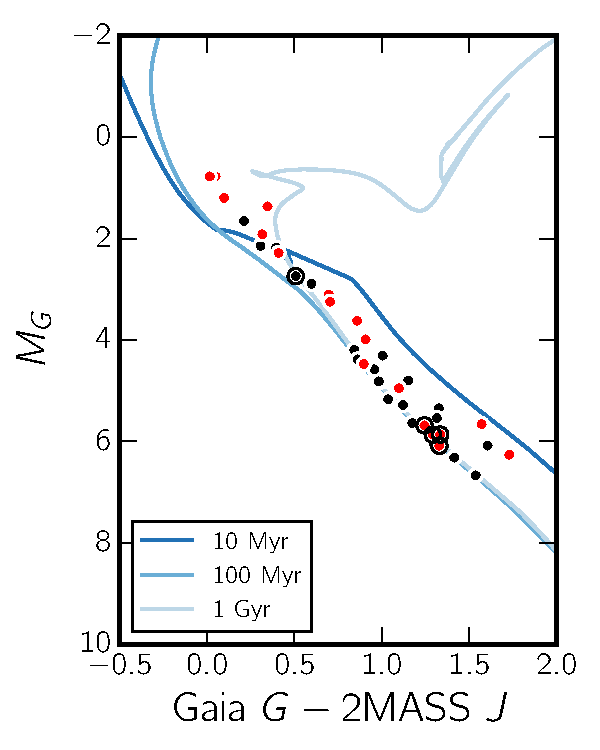
\includegraphics[width=0.7\linewidth]{cmd_gjg.pdf}
%   \caption{Color-magnitude diagram of member stars.
%     For comparison, we show the MIST isochrones of a solar metallicity population \todo{cite mist}.
%     Red markers indicate infrared excess,
%     and markers wrapped in black circles indicate X-ray source (Table~\todo{tablenum}).
%   }
%   \label{fig:cmd_gjg}
% \end{figure}

\acknowledgements
% simbad
This research has made use of the SIMBAD database,
operated at CDS, Strasbourg, France.
% ads
This research has made use of NASA's Astrophysics Data System.
% gaia
% gaia sprints


\bibliography{refs}

\end{document}
